% Chapter 1

\chapter{État de l'art et fondements théoriques} % Chapter title

\label{ch:1} % For referencing the chapter elsewhere, use \autoref{ch:1} 

\section{Généralités sur l'intelligence artificielle}

L'\acf{ia} peut être définie de diverses manières, mais une définition largement acceptée la décrit comme la création de systèmes informatiques capables d'accomplir des tâches qui nécessitent normalement l'intelligence humaine, telles que la reconnaissance de formes, la compréhension du langage, l'apprentissage et le raisonnement \cite{Goodfellow-et-al-2016, Caelen_Blete_2023}.

Cette capacité à simuler des processus cognitifs humains est rendue possible grâce à une branche spécifique appelée "\acf{ml}". Celle-ci permet aux ordinateurs d'apprendre à partir de données c'est à dire : d'identifier des motifs et de prendre des décisions. 

Le \acs{ml} repose donc sur la conception d'algorithmes \footnote{"Un algorithme est une suite finie et non ambiguë d'instructions et d’opérations permettant de résoudre une classe de problèmes." \cite{frwiki:213207404}} capables d'accéder à des données et de les utiliser pour se former eux-mêmes à accomplir des tâches spécifiques. Cette conception table sur une solide base mathématique et statistique, qui fournit les outils nécessaires pour modéliser et comprendre les motifs complexes dans les données. Les données traitées sont souvent représentées sous forme de matrices. Par exemple, une image peut être représentée comme une matrice de pixels, où chaque élément de la matrice correspond à la valeur d'un pixel (voir Figure~\ref{fig:mnist-image-matrix}). 

\begin{figure}[H]
    \centering
    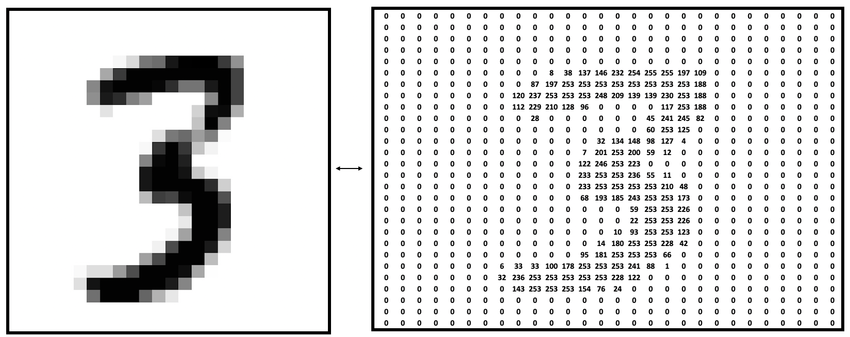
\includegraphics[width=8cm]{gfx/fig-mnist-image-matrix.png}
    \caption{Représentation de la valeur trois dans l'ensemble de données MNIST et sa matrice équivalente \cite{mnist}.}
    \label{fig:mnist-image-matrix}
\end{figure}

De même, les opérations sur les données, telles que les transformations appliquées par les couches d'un réseau de neurones, sont effectuées à l'aide d'opérations d'algèbre linéaire sur ces matrices.

L'inférence \footnote{"Opération logique par laquelle on admet une proposition en vertu de sa liaison avec d'autres propositions déjà tenues pour vraies." - Le Robert} statistique quant à elle permet aux algorithmes de faire des prédictions sur des données non vues auparavant, en se basant sur les probabilités extraites de l'ensemble de données d'apprentissage. Cela signifie que si un modèle est entraîné avec suffisamment de données représentatives, il peut inférer des résultats pour de nouvelles données basées sur les motifs appris \cite{Deisenroth_Faisal_Ong_2020}.

En combinant l'inférence statistique avec l'algèbre linéaire, les algorithmes de \ac{ml} peuvent donc apprendre à partir de données complexes, identifier des motifs subtils et faire des prédictions précises.  

\subsection{Le modèle}

Dans ce contexte un modèle peut être défini comme une abstraction mathématique, un ensemble d'équations, ou un algorithme conçu pour effectuer une tâche spécifique. Ce modèle est formé à partir de données et apprend à effectuer cette tâche en identifiant des motifs, des relations, ou des structures au sein des données. Les modèles peuvent varier grandement en complexité, depuis des modèles linéaires simples jusqu'à des réseaux de neurones profonds très complexes \cite{Deisenroth_Faisal_Ong_2020}.

Un modèle de \ac{ml} est composé de trois composants principaux :

\begin{itemize}
    \item \textbf{L'architecture du modèle} : C'est la structure sous-jacente du modèle, qui définit la manière dont les données d'entrée sont transformées en sorties. Par exemple, dans un réseau de neurones, l'architecture inclurait le nombre de couches cachées, le nombre de neurones dans chaque couche, le type d'activation utilisé, etc.

    \item \textbf{Les paramètres du modèle} : Ce sont les éléments du modèle qui sont ajustés au cours de l'entraînement pour minimiser la fonction d'erreur. Dans un réseau de neurones, les paramètres sont les poids et les biais associés à chaque connexion entre les neurones. Dans une régression linéaire, les paramètres seraient le coefficient de pente et l'ordonnée à l'origine. Par exemple :

    \begin{equation}
        y = mx + b
    \end{equation}

    Où :

    \begin{itemize}
        \item $y$ est la variable dépendante ou la sortie que l'on souhaite de prédire ou d'expliquer.
        
        \item $x$ est la variable indépendante ou l'entrée pour faire des prédictions.
        
        \item $m$ est le coefficient de pente, qui représente la variation attendue dans  $y$ pour une variation d'une unité dans $x$.  En d'autres termes, il quantifie l'effet de la variable indépendante sur la variable dépendante.
    
        \item $b$ est l'ordonnée à l'origine, qui représente la valeur de $y$ lorsque $x$ est égal à zéro. C'est là où la ligne de régression coupe l'axe des ordonnées.
    \end{itemize}
    
    $m$ et $b$ sont les paramètres du modèle de régression linéaire. Pendant le processus d'entraînement, ces paramètres sont ajustés pour minimiser la différence entre les valeurs prédites par le modèle et les valeurs réelles des données d'entraînement. Cette différence est souvent mesurée en utilisant la somme des carrés des résidus ou une autre fonction de perte similaire \cite{Bonaccorso_2018}.

    \item \textbf{L'algorithme d'apprentissage} : C'est la méthode utilisée pour ajuster les paramètres du modèle en fonction des données d'entrée et de la fonction d'erreur. L'algorithme d'apprentissage spécifie comment le modèle est entraîné, par exemple, en utilisant la descente de gradient pour minimiser la fonction d'erreur.
\end{itemize}

L'objectif d'un modèle est de généraliser à partir des données d'entraînement, c'est-à-dire d'être capable de faire des prédictions précises ou de prendre des décisions judicieuses sur de nouvelles données, jamais vues auparavant. La capacité d'un modèle à bien généraliser est essentielle pour son efficacité dans des applications réelles. La généralisation est souvent évaluée en utilisant un ensemble de données de test distinct de l'ensemble de données d'entraînement, permettant d'estimer la performance du modèle dans le monde réel \cite{Bonaccorso_2018, Deisenroth_Faisal_Ong_2020}.

\subsection{L'apprentissage}

L'apprentissage est un processus itératif qui se fait au travers de ce qu'on appelle des "epochs" - chaque epoch \footnote{"le nombre de passages d'un dataset d'entraînement par un algorithme. Un passage équivaut à un aller-retour. Le nombre d'epochs peut atteindre plusieurs milliers, car la procédure se répète indéfiniment jusqu'à ce que le taux d'erreurs du modèle soit suffisamment réduit." \cite{Kassel_2023}} représentant un cycle complet de passage de l'ensemble des données d'apprentissage à travers le modèle. Pour évaluer et affiner la performance du modèle, les données sont généralement subdivisées en deux ou trois catégories : un ensemble d'entraînement (train), un ensemble de test, et parfois un ensemble de validation. 

\begin{figure}[H]
    \centering
    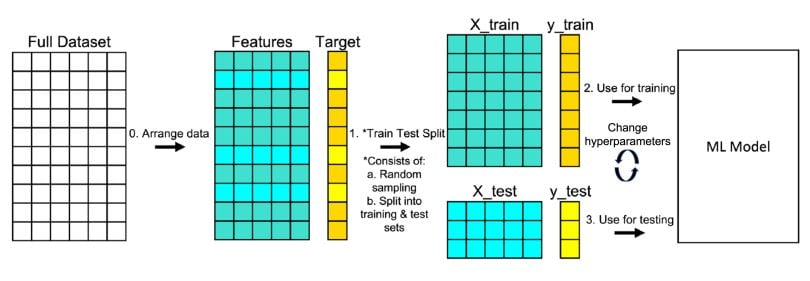
\includegraphics[width=15cm]{gfx/fig-dataset-split.jpg}
    \caption{
       Procédure de subdivision du dataset. | Image : Michael Galarnyk
    }
    \label{fig:mlprocess}
\end{figure}

L'ensemble d'entraînement sert à ajuster les paramètres du modèle, tandis que l'ensemble de test est utilisé pour évaluer sa performance. L'ensemble de validation, lorsqu'il est présent, aide à affiner les hyperparamètres \footnote{paramètres qui définissent la structure du modèle et son comportement, comme le taux d'apprentissage} du modèle et à éviter le surapprentissage \footnote{"Le surajustement est un comportement indésirable d'apprentissage automatique qui se produit lorsque le modèle d'apprentissage automatique fournit des prédictions précises pour les données d'entraînement mais pas pour les nouvelles données." \cite{overfitting}} en fournissant une couche d'évaluation supplémentaire avant le test final. Tout au long de ce processus, tant les hyperparamètres que les paramètres \footnote{poids et biais ajustés au cours de l'apprentissage} sont ajustés et optimisés dans le but de minimiser l'erreur de prédiction du modèle. Cet ajustement méthodique assure une amélioration continue de la performance du modèle, le rendant de plus en plus précis dans ses prédictions ou classifications sur des données non vues auparavant.


Les types d'apprentissage en \ac{ml} sont généralement classés en trois grandes catégories :

\begin{itemize}
    \item \textbf{Apprentissage supervisé} : Dans cette approche, le modèle apprend à partir d'un ensemble de données étiqueté, où chaque exemple d'entraînement comprend des entrées et les sorties correspondantes. Le but est de permettre au modèle de prédire la sortie associée à de nouvelles entrées inédites. Des exemples classiques incluent la régression linéaire et la classification.

    \begin{figure}[H]
        \centering
        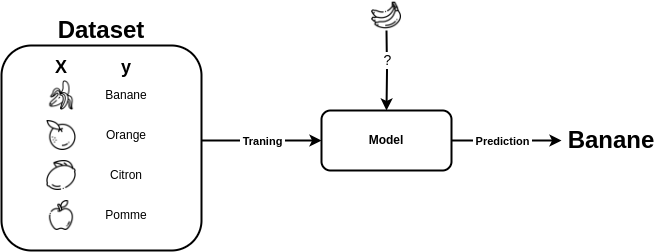
\includegraphics[width=10cm]{gfx/fig-supervised-learning.png}
        \caption{Apprentissage supervisé.}
        \label{fig:supervised-learning}
    \end{figure}

    \item \textbf{Apprentissage non supervisé} : Ici, le modèle travaille sur des données non étiquetées, apprenant à identifier les structures et les motifs inhérents sans aucune indication de sortie désirée. Les algorithmes d'apprentissage non supervisé, tels que le clustering ou la réduction de dimensionnalité, visent à découvrir des groupements naturels dans les données ou à simplifier les données tout en conservant leur structure essentielle.

    \begin{figure}[H]
        \centering
        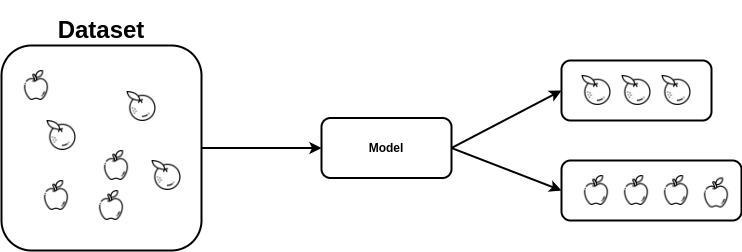
\includegraphics[width=10cm]{gfx/fig-unsupervised-learning.png}
        \caption{Apprentissage non supervisé.}
        \label{fig:unsupervised-learning}
    \end{figure}

    \item \textbf{Apprentissage par renforcement} : Dans l'apprentissage par renforcement, un agent apprend à prendre des décisions en exécutant des actions dans un environnement afin de maximiser une certaine notion de récompense cumulative. C'est une approche dynamique où l'apprentissage est guidé par les interactions de l'agent avec l'environnement et les retours (récompenses) reçus pour ses actions.

    \begin{figure}[H]
        \centering
        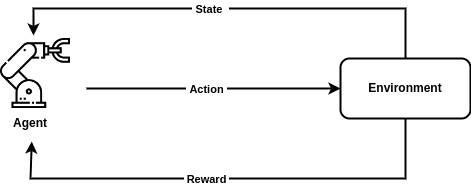
\includegraphics[width=10cm]{gfx/fig-reinforcement-learning.png}
        \caption{Apprentissage par renforcement.}
        \label{fig:reinforcement-learning}
    \end{figure}
\end{itemize}

Ces différents types d'apprentissage sont adaptés à diverses tâches. Ces tâches peuvent être regroupées en plusieurs catégories principales, chacune répondant à des objectifs spécifiques et utilisant des types de modèles appropriés. Voici une énumération de certaines des tâches les plus communes, comme détaillé par Giuseppe Bonaccorso dans \cite{Bonaccorso_2018} :

\begin{enumerate}
    \item Régression
    
    La régression vise à prédire une valeur continue ou quantitative basée sur une ou plusieurs variables indépendantes. Elle est souvent utilisée pour estimer des phénomènes tels que les prix des logements, les températures futures, ou les niveaux de vente. Les types de régression incluent :
    
    \begin{itemize}
        \item Régression linéaire
        \item Régression polynomiale
        \item Régression par arbre de décision
        \item Régression Ridge/Lasso
        \item Classification
    \end{itemize}    

    \item Classification
    
    La classification concerne la prédiction d'une catégorie ou classe discrète pour une observation. Elle est utilisée dans des tâches telles que la détection de spams, la reconnaissance d'images, et le diagnostic médical. Les algorithmes de classification incluent :

        \begin{itemize}
            \item Réseaux de neurones
            \item \ac{svm}
            \item Forêts aléatoires
            \item \ac{knn}
            \item Classificateurs bayésiens naïfs
        \end{itemize}

    \item Clustering
    
    Le clustering (ou regroupement) a pour but de diviser les données en groupes, ou clusters, de sorte que les points de données dans le même groupe soient plus similaires les uns aux autres qu'aux points dans d'autres groupes. Il est utilisé pour l'analyse exploratoire des données, la segmentation de marché, et l'organisation de grandes bases de données. Les méthodes de clustering comprennent :

       \begin{itemize}
            \item K-means
            \item Clustering hiérarchique
            \item \ac{dbscan}
            \item Clustering basé sur la densité
       \end{itemize}

    \item Détection d'anomalies
    
    La détection d'anomalies (ou détection d'outliers) identifie les observations qui dévient significativement du reste des données. Elle est cruciale dans des domaines tels que la détection de fraude, la surveillance de la santé des systèmes et la maintenance prédictive. Les techniques courantes incluent :

       \begin{itemize}
            \item Isolation Forest
            \item One-Class \acs{svm}
            \item Méthodes basées sur la proximité
       \end{itemize}

    \item Réduction de dimensionnalité
    
    La réduction de dimensionnalité consiste à diminuer le nombre de variables aléatoires sous-jacentes, ou dimensions, dans un ensemble de données. Cela peut aider à améliorer l'efficacité des algorithmes d'apprentissage et à visualiser les données. Les approches incluent :

        \begin{itemize}
            \item \ac{pca}
            \item \ac{tsne}
            \item Auto-encodeurs (dans le cadre de l'apprentissage profond)
        \end{itemize}
\end{enumerate}

Chacune de ces tâches exploite des principes et des algorithmes d'apprentissage automatique pour interpréter les données et faire des prédictions ou des classifications. Le choix de la tâche et de l'algorithme dépend largement du problème spécifique à résoudre et de la nature des données disponibles \cite{ml_task, Flach_2012}.

Ce tableau n'est pas exhaustif mais donne un aperçu général des associations entre les types d'apprentissage, les tâches spécifiques, et les algorithmes.

\begin{table}[h]
\centering
\begin{tabular}{|l|l|l|}
    \hline
    \textbf{Type d'apprentissage} & \textbf{Tâche}             & \textbf{Algorithmes}                       \\ \hline
    Supervisé                     & Régression                 & Régression linéaire, Forêts aléatoires     \\ \cline{2-3} 
                                  & Classification             & \ac{svm}, \ac{knn}, Réseaux de neurones             \\ \hline
    Non supervisé                 & Clustering                 & K-means, Clustering hiérarchique           \\ \cline{2-3} 
                                  & Réduction de dimensionnalité & \ac{pca}, \ac{tsne}                               \\ \cline{2-3}
                                  & Détection d'anomalies      & Isolation Forest, One-Class \ac{svm}            \\ \hline
    Par renforcement              & Prise de décision         & Q-learning, \ac{dqn}            \\ \hline
\end{tabular}
\caption{Association entre types d'apprentissage, tâches et algorithmes en \ac{ml}}
\label{table:mapping-type-task-algorithms}
\end{table}

\subsection{Le processus de l'apprentissage automatique} \hspace{0pt}
\label{ch:1:section:ml-process}

\begin{figure}[H]
    \centering
    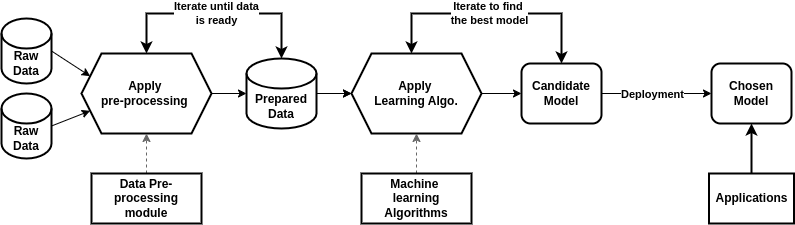
\includegraphics[width=15cm]{gfx/fig-machine-learning-process.png}
    \caption{Le processus de l'apprentissage automatique \cite{mlprocess}.}
    \label{fig:mlprocess}
\end{figure}

L'apprentissage est dit "automatique" en raison de la capacité des modèles à apprendre à partir de données sans intervention humaine explicite après leur programmation initiale. Comme nous pouvons le voir sur la figure~\ref{fig:mlprocess}, le processus de développement d'un modèle d'apprentissage automatique est présenté comme un flux de travail structuré en plusieurs étapes clés :

\begin{enumerate}
    \item Tout commence avec les données brutes, ces données peuvent provenir de différentes sources et sont souvent hétérogènes, non structurées et peuvent contenir des erreurs ou des valeurs manquantes.

    \item Les données brutes subissent un processus de pré-traitement, qui peut inclure le nettoyage, la normalisation, la transformation et la sélection des caractéristiques. Cette étape est cruciale pour préparer les données de manière à ce qu'elles puissent être utilisées efficacement par les algorithmes d'apprentissage automatique. Le pré-traitement est souvent un processus itératif, comme l'indique la flèche retournant vers la boîte de pré-traitement.

    \item Après le pré-traitement, les données sont prêtes à être utilisées dans des modèles d'apprentissage automatique. Ces données préparées sont généralement plus propres, pertinentes et formatées de manière appropriée pour l'entraînement des modèles.

    \item Les données préparées sont ensuite utilisées pour entraîner différents modèles à l'aide de divers algorithmes d'apprentissage automatique. Cette étape peut impliquer l'utilisation de techniques d'apprentissage supervisé, non supervisé ou par renforcement, selon la nature de la tâche à accomplir.

    \item Plusieurs modèles candidats sont généralement produits et évalués pour déterminer lequel performe le mieux selon les critères de succès définis pour le projet. Ce processus peut nécessiter de nombreuses itérations pour affiner et optimiser les modèles.

    \item Le modèle qui présente les meilleures performances est sélectionné comme le modèle final. C’est ce modèle qui sera déployé dans une application réelle.

    \item Une fois le modèle choisi, il est déployé dans l'environnement de production où il peut être utilisé pour effectuer la tâche pour laquelle il a été conçu, comme faire des prédictions, classer des données ou automatiser des décisions.

    \item Finalement, le modèle déployé est intégré à des applications ou systèmes plus larges, où il peut fournir une valeur ajoutée, comme améliorer l'expérience utilisateur, augmenter l'efficacité opérationnelle ou générer des perspectives à partir des données.
\end{enumerate}


\subsection{L'apprentissage profond}

\begin{figure}[H]
    \centering
    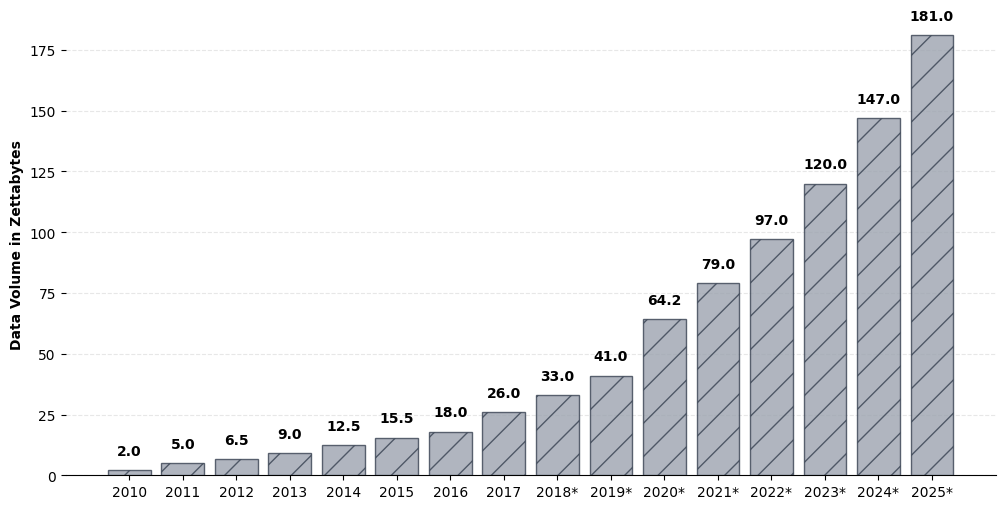
\includegraphics[width=15cm]{gfx/fig-big-data.png}
    \caption{Volume de données/informations créées, capturées, copiées et consommées dans le monde de 2010 à 2020, avec des prévisions de 2021 à 2025. (Voir code~\ref{appendix:code:python:plot-generation}) \cite{datagenerate2010}.}
    \label{fig:datagenerated}
\end{figure}

L'avènement d'Internet a entraîné une explosion de la quantité de données générées, connue sous le nom de "big data". Le big data désigne de vastes ensembles de données si complexes et volumineux qu'ils sont difficiles à traiter avec des outils de gestion de base de données traditionnels \cite{Ratner_2012}.

Ces données, provenant de diverses sources telles que les médias sociaux, les transactions en ligne, les capteurs et les dispositifs connectés, représentent une mine d'or pour l'entraînement des modèles de \ac{ml}, offrant une richesse d'informations pour améliorer la précision des prédictions et des décisions.

Cependant, l'apprentissage automatique traditionnel s'est avéré insuffisant pour traiter efficacement le volume, la variété et la vélocité du big data. 

Cela a conduit à l'émergence de l'\acf{dl}, un sous-ensemble de l'apprentissage automatique qui utilise des réseaux de neurones artificiels profonds. Le \ac{dl} s'inspire de la structure et du fonctionnement du cerveau humain, permettant aux modèles de traiter des niveaux de complexité et de subtilité dans les données bien au-delà de la portée des approches traditionnelles de \ac{ml}. Grâce à sa capacité à apprendre des caractéristiques hiérarchiques dans les données, le deep learning s'est avéré particulièrement efficace pour des tâches complexes telles que la reconnaissance d'images, la compréhension du langage naturel et la génération de contenu créatif \cite{Foster_2019}.

\begin{figure}[H]
    \centering
    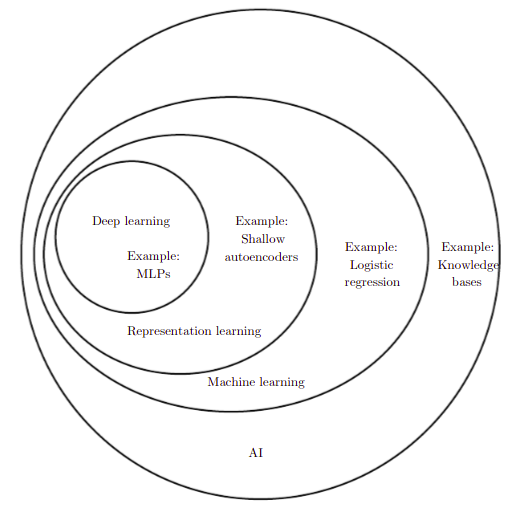
\includegraphics[width=12cm]{gfx/fig-dl-ml-ai.png}
    \caption{Un diagramme de Venn montrant comment l'apprentissage profond est lié à l'apprentissage par représentation, qui est à son tour lié à l'apprentissage automatique, qui est utilisé dans plusieurs approches de L'\ac{ia}, mais pas toutes \cite{Goodfellow-et-al-2016}}.
    \label{fig:dl-ml-ai}
\end{figure}

L'apprentissage profond s'appuie sur une représentation mathématique spécifique du cerveau humain, connue sous le nom de réseaux de neurones. Ces réseaux forment le cœur des algorithmes d'apprentissage profond et sont responsables de leur capacité à apprendre des modèles complexes dans d'immenses ensembles de données. 

\subsubsection{Le perceptron}

\begin{figure}[H]
    \centering
    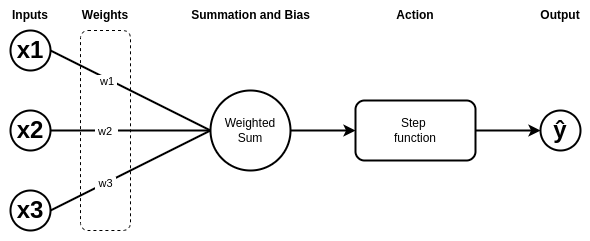
\includegraphics[width=12cm]{gfx/fig-perceptron.png}
    \caption{Le perceptron}.
    \label{fig:perceptron}
\end{figure}

Le perceptron peut être considéré comme la brique élémentaire des réseaux de neurones. Développé dans les années 1950 par Frank Rosenblatt \footnote{"Frank Rosenblatt (né à New Rochelle le 11 juillet 1928 - mort le 11 juillet 1971) est un psychologue américain qui travaille sur l'intelligence artificielle. Principal représentant du « courant neuronal », qui voulait construire celle-ci à partir de la conception du réseau neuronal humain, il développe sur ce modèle le perceptron en 1957 à l'Université Cornell." \cite{frwiki:213039317}}, il représente un modèle simplifié d'un neurone biologique. Un perceptron reçoit plusieurs entrées, chacune d'elles étant pondérée par un poids spécifique. Ces entrées pondérées sont ensuite sommées, et si la somme dépasse un certain seuil, le perceptron émet un signal de sortie. Cette sortie est déterminée par une fonction d'activation, qui, dans le cas du perceptron initial, est typiquement une fonction d'étape. Le perceptron ajuste ses poids à travers un processus d'apprentissage basé sur les erreurs commises, raffinant ainsi sa capacité à classer correctement les entrées \cite{wang2017origin}.

Bien que le perceptron ait marqué un tournant dans le développement des algorithmes d'apprentissage automatique, il présente des limitations, notamment son incapacité à traiter des problèmes non linéairement séparables, comme l'opérateur logique XOR (voir Figure~\ref{fig:perceptron-xor}). Cette limitation a conduit à l'exploration de structures plus complexes, ouvrant la voie aux réseaux de neurones  \cite{Min69}.

\begin{figure}[H]
    \centering
    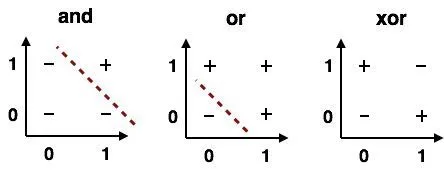
\includegraphics[width=8cm]{gfx/fig-perceptron-xor.png}
    \caption{XOR est considéré comme non-linéaire du fait qu'aucune ligne droite ne peut séparer les sorties de 0 et de 1 dans un espace bidimensionnel où les axes représentent les entrées. \cite{Jaspreet_2022}}.
    \label{fig:perceptron-xor}
\end{figure}

\subsubsection{Les réseaux de neurones}

Un réseau de neurones, dans son essence, est une collection de perceptrons (ou neurones artificiels) organisés en couches. Un réseau typique comprend une couche d'entrée, une ou plusieurs couches cachées, et une couche de sortie. Chaque neurone dans une couche est connecté à plusieurs neurones dans la couche suivante, permettant ainsi au réseau de traiter l'information de manière hiérarchique. Ce design permet aux réseaux de neurones d'apprendre des relations complexes et non linéaires dans les données \cite{Jaspreet_2022, Min69}.

\begin{figure}[H]
    \centering
    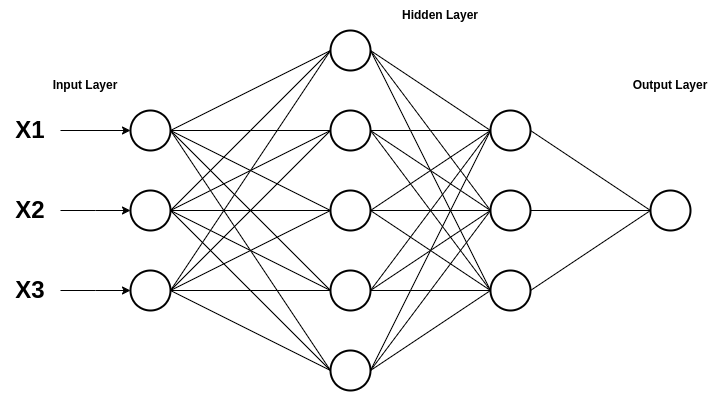
\includegraphics[width=12cm]{gfx/fig-nn.png}
    \caption{Un réseaux de neurones}.
    \label{fig:perceptron}
\end{figure}

Les réseaux de neurones sont entraînés à l'aide d'algorithmes d'optimisation, comme la descente de gradient, qui ajustent les poids des connexions neuronales afin de minimiser l'erreur entre les prédictions du réseau et les véritables valeurs \cite{antoine2018apprentissage}.

Ce tableau n'est pas exhaustif mais donne un aperçu général des associations entre les types d'apprentissage, les tâches spécifiques, et architectures.

\begin{table}[h]
\centering
\begin{tabular}{|l|l|l|}
\hline
\textbf{Tâche}                   & \textbf{Architecture NN}                     & \textbf{Type d'apprentissage}   \\ \hline
Classification          & MLP, CNN, RNN, LSTM, Transformers   & Supervisé                \\ \hline
Régression              & MLP, CNN                              & Supervisé                \\ \hline
Clustering              & Auto-encodeurs, SOM                  & Non supervisé            \\ \hline
Réduction de dimension  & Auto-encodeurs, PCA Neural Network   & Non supervisé            \\ \hline
Détection d'anomalies   & Auto-encodeurs, One-Class NN         & Non supervisé            \\ \hline
Prise de décision       & DQN, Policy Gradient, Actor-Critic   & Par renforcement         \\ \hline
\end{tabular}
\caption{Association entre tâches, architectures de modèles NN et type d'architectures}
\label{tab:my-table}
\end{table}

\newpage
\paragraph{L'optimisation} \hspace{0pt}

\begin{figure}[H]
    \centering
    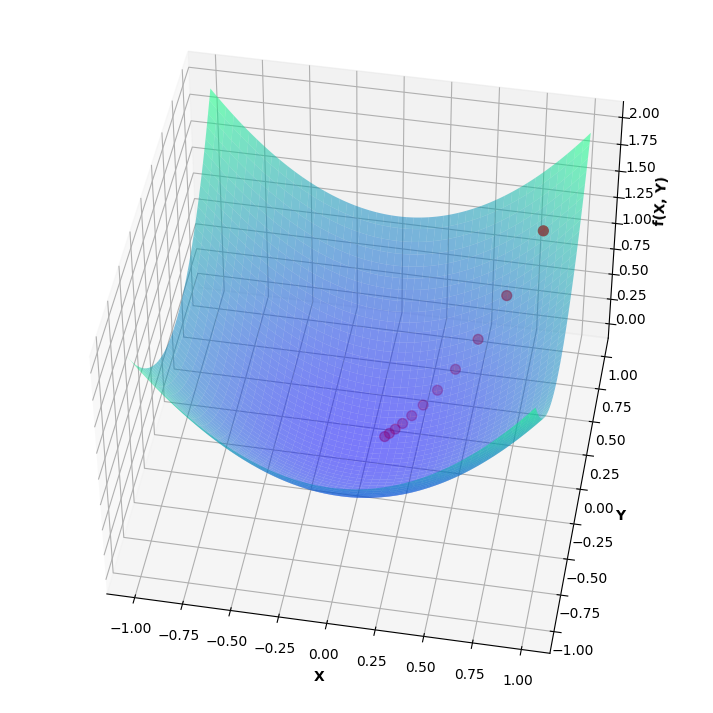
\includegraphics[width=8cm]{gfx/fig-gradient-descent.png}
    \caption{\acf{gd} (voir Code~\ref{appendix:code:python:gd})}
    \label{fig:gradient-descent}
\end{figure}

Les réseaux de neurones utilisent plusieurs algorithmes d'optimisation pour minimiser la fonction de perte durant l'entraînement. Ces algorithmes ajustent les poids du réseau de manière itérative pour réduire au minimum la différence entre les prédictions et les vraies valeurs. Voici une liste des algorithmes d'optimisation les plus utilisés, accompagnés de leurs formules de base \cite{ruder2016overview, Goodfellow-et-al-2016} :

\begin{itemize}
    \item \acf{gd}
    \begin{equation}
        \theta = \theta - \eta \cdot \nabla_\theta J( \theta)
    \end{equation}
    Mise à jour des paramètres en soustrayant le produit du taux d'apprentissage \( \eta \) et du gradient de la fonction de coût \( J(\theta) \) par rapport aux paramètres \( \theta \).

    \item \acf{sgd}
    \begin{equation}
        \theta = \theta - \eta \cdot \nabla_\theta J( \theta; x^{(i)}; y^{(i)})
    \end{equation}
    Similaire à \ac{gd}, mais la mise à jour est faite pour chaque exemple d'entraînement. Cela rend \ac{sgd} plus rapide et capable de s'échapper des minima locaux.
    
    \item \acf{sgd} avec Momentum
    \begin{align}
    \begin{split}
        v_t &= \gamma v_{t-1} + \eta \nabla_\theta J( \theta)\\
        \theta &= \theta - v_t
    \end{split}
    \end{align}
    Ajoute une fraction \( \gamma \) du vecteur de mise à jour précédent à la mise à jour courante pour accélérer la convergence.
    
    \item \acf{adagrad}
    \begin{align}
    \begin{split}
        g_{t, i} &= \nabla_{\theta_t} J( \theta_{t,i} ) \\
        \theta_{t+1, i} &= \theta_{t, i} - \eta \cdot g_{t, i} \\
        \theta_{t+1, i} &= \theta_{t, i} - \frac{\eta}{\sqrt{G_{t, ii} + \epsilon}} \cdot g_{t, i}
    \end{split}
    \end{align}
    
    Adapte le taux d'apprentissage à chaque paramètre en divisant par la racine carrée de la somme des carrés des gradients précédents. \( G_t \) est une matrice diagonale où chaque élément diagonal est la somme des carrés des gradients pour un paramètre spécifique, et \( \epsilon \) est un terme de lissage pour éviter la division par zéro.
    
    \item \acf{rmsprop}
    \begin{align}
    \begin{split}
        E[g^2]_t &= 0.9 E[g^2]_{t-1} + 0.1 g^2_t \\
        \theta_{t+1} &= \theta_{t} - \frac{\eta}{\sqrt{E[g^2]_t + \epsilon}} g_{t}
    \end{split}
    \end{align}
    
    Modifie \ac{adagrad} pour améliorer ses performances avec des gradients très différents en utilisant une moyenne mobile exponentielle du carré des gradients.
    
    \item \acf{adam}
    \begin{align}
    \begin{split}
        m_t &= \beta_1 m_{t-1} + (1 - \beta_1) g_t \\
        v_t &= \beta_2 v_{t-1} + (1 - \beta_2) g_t^2 \\
        \hat{m}_t &= \frac{m_t}{1 - \beta^t_1} \\
        \hat{v}_t &= \frac{v_t}{1 - \beta^t_2} \\
        \theta_{t+1} &= \theta_{t} - \frac{\eta}{\sqrt{\hat{v}_t} + \epsilon} \hat{m}_t
    \end{split}
    \end{align}
    Calcule des moyennes mobiles exponentielles des gradients et des carrés des gradients. Les estimations sont corrigées pour obtenir des estimations non biaisées, ce qui améliore l'efficacité de l'algorithme dans les premiers temps de l'optimisation.
\end{itemize}

Dans le cadre de ce mémoire, nous ne nous concentrerons pas sur les aspects mathématiques sous-jacents des algorithmes d'optimisation ni sur les diverses architectures de réseaux de neurones. Comme souligné précédemment, notre intérêt se porte principalement sur le traitement du langage humain et son application dans le développement de chatbots.

\subsection{Les \acfp{llm}}
\label{ch:1:section:llm}

Un modèle de langage (LM) est un type de modèle utilisé dans le domaine du \ac{nlp} pour comprendre, générer, et manipuler le langage humain. À son essence, un LM apprend la structure et les règles d'une langue à partir de grandes quantités de texte, permettant ainsi de prédire le mot suivant dans une phrase donnée, de générer du texte cohérent, ou d'accomplir d'autres tâches liées au langage \cite{Jurafsky2009}. 

Les modèles de langage sont entraînés à comprendre les probabilités d'apparition des mots ou des séquences de mots dans une langue. Initialement, des approches plus simples comme les modèles n-grammes étaient utilisées, où la prédiction du mot suivant se basait uniquement sur les n-1 mots précédents, sans tenir compte du contexte global ou des nuances sémantiques plus larges \cite{Jurafsky2009, Agarwal}.

\begin{figure}[H]
    \centering
    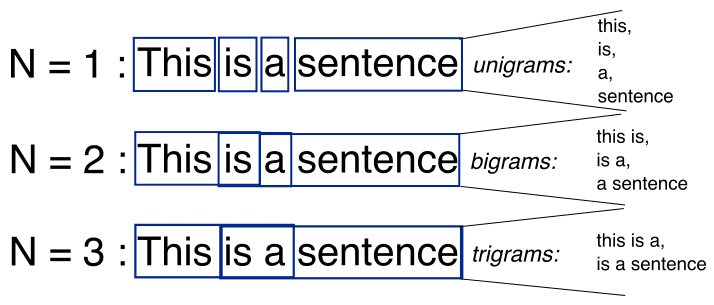
\includegraphics[width=12cm]{gfx/fig-n-gram.png}
    \caption{Modèle uni-gramme, bi-gramme et tri-gramme. \cite{Agarwal}}
    \label{fig:n-gram}
\end{figure}

Prenons l'exemple d'un modèle trigramme (un cas spécifique où $n = 3$) pour illustrer comment cela fonctionne, Considérons la phrase "Le chat mange". Si nous voulons prédire le mot suivant après "chat mange", un modèle tri-gramme regardera les occurrences de "chat mange" dans le corpus\footnote{"Un corpus est un ensemble de documents, artistiques ou non, regroupés dans une optique précise. On peut utiliser des corpus dans plusieurs domaines : études littéraires, linguistiques, scientifiques, philosophie, etc." \cite{frwiki:205358830}} d'entraînement et calculera la probabilité du mot suivant chaque occurrence.

La probabilité d'un mot \(w_n\) sachant les deux mots précédents \(w_{n-2}\) et \(w_{n-1}\) dans un modèle trigramme est donnée par : 

\begin{equation}
    P(w_n | w_{n-2}, w_{n-1}) = \frac{C(w_{n-2}, w_{n-1}, w_n)}{C(w_{n-2}, w_{n-1})}
\end{equation}

où :
\begin{itemize}
    \item[--] \(P(w_n | w_{n-2}, w_{n-1})\) est la probabilité conditionnelle du mot \(w_n\) sachant les deux mots précédents \(w_{n-2}\) et \(w_{n-1}\).
    \item[--] \(C(w_{n-2}, w_{n-1}, w_n)\) est le nombre d'occurrences de la séquence de trois mots \(w_{n-2}, w_{n-1}, w_n\) dans le corpus d'entraînement.
    \item[--] \(C(w_{n-2}, w_{n-1})\) est le nombre d'occurrences de la séquence de deux mots \(w_{n-2}, w_{n-1}\) dans le corpus.
\end{itemize}

Les mathématiques sous-jacentes du n-gramme ont été proposées pour la première fois par Markov (1913) dans \cite{Markov}.

En contraste, les \acfp{llm} utilisent des réseaux de neurones profonds pour apprendre à partir de vastes ensembles de données textuelles, leur permettant de capturer des nuances linguistiques et des dépendances complexes. Au cœur de ces modèles se trouve souvent l'architecture Transformer (voir Section~\ref{ch:1:section:transformer}), qui, grâce à son mécanisme d'attention, permet de considérer l'intégralité du texte en entrée, offrant une compréhension bien plus riche du contexte et des relations à longue distance.

Ces modèles sont dits "à grande échelle" parce qu'ils sont entraînés sur d'immenses volumes de données, ce qui leur permet de prédire le mot suivant en considérant tout le contexte donné. Leur performance dépend également du nombre de leurs paramètres, souvent en milliards, reflétant leur capacité à mémoriser et générer du langage. Plus un modèle a de paramètres, mieux il peut gérer un contexte étendu, ce qui améliore sa compréhension du langage et sa capacité à saisir les nuances \cite{Caelen_Blete_2023}.

\subsubsection{Les modèles open-source}

Après l'entraînement, les poids de ces modèles sont sauvegardés et souvent hébergés sur des plateformes de partage et de collaboration comme Hugging Face\footnote{\href{https://huggingface.co/}{https://huggingface.co/}}, où ils deviennent accessibles à tous.

Les poids des modèles open-source peuvent être exécutés par quiconque en utilisant des outils et des librairies adaptés, tels que Ollama \footnote{\href{https://github.com/ollama/}{https://github.com/ollama/}} ou llama.cpp\footnote{\href{https://github.com/ggerganov/llama.cpp}{https://github.com/ggerganov/llama.cpp}}. Ces outils facilitent l'implémentation des modèles de langage dans divers environnements et applications, permettant une grande variété d'usages.

\begin{table}[H]
\centering
\begin{tabular}{|l|p{12cm}|}
\hline
\textbf{Modèle} & \textbf{Description} \\ \hline
gemma & Gemma est une famille de modèles ouverts légers et de pointe construits par Google DeepMind \cite{gemma_2024}. \\ \hline
llama2  & Llama 2 est une collection de modèles linguistiques de base allant des paramètres 7B à 70B \cite{touvron2023llama}. \\ \hline
mistral & Le modèle 7B publié par Mistral AI, mis à jour à la version 0.2 \cite{jiang2023mistral}. \\ \hline
Vicuna & Modèle de chat à usage général basé sur Llama et Llama 2 avec des contextes de 2K à 16K \cite{vicuna2023}. \\ \hline
Starling & formé par apprentissage par renforcement à partir du retour d'information de L'\ac{ia}, qui vise à améliorer l'utilité des chatbots. \cite{starling2023}. \\ \hline
mixtral & Un modèle de mélange d'experts (MoE) de haute qualité avec des poids ouverts par Mistral AI. \\ \hline
llava & LLaVA est un nouveau modèle multimodal entraîné de bout en bout qui combine un encodeur de vision et Vicuna \\ \hline
\end{tabular}
\caption{Principaux modèles Open source}
\label{table:llm-models}
\end{table}


\subsubsection{Les modèles entreprise}

D'autre part, les modèles d'entreprise sont développés comme des services disponibles via des \acs{api} payantes ou pas, ce qui représente un modèle d'accès différent par rapport aux modèles open-source. Ces \acs{api} offrent aux entreprises la possibilité d'intégrer des capacités d'intelligence artificielle avancées dans leurs propres systèmes et applications, sans avoir à supporter directement les coûts et la complexité liés à l'entraînement, au déploiement, et à la maintenance de ces modèles.
 
\begin{table}[H]
\centering
\begin{tabular}{|l|p{14cm}|}
\hline
\textbf{Modèle} & \textbf{Description} \\ \hline
GPT-4 & La suite de GPT-3, GPT-4 améliore les capacités de génération de texte et de compréhension du modèle avec un nombre encore plus grand de paramètres \cite{openai2023gpt4}. \\ \hline
Gemini & Le modèle créé par Google avec 137B paramètres \cite{geminiteam2023gemini}. \\ \hline
\end{tabular}
\caption{Principaux modèles Entreprise}
\label{table:llm-models-closed}
\end{table}




% %---------------------------------------------------------------------------------------%
\newpage
\subsection{l'architecture Transformer \cite{Caelen_Blete_2023, vaswani2023attention}}
\label{ch:1:section:transformer}

\begin{figure}[H]
    \centering
    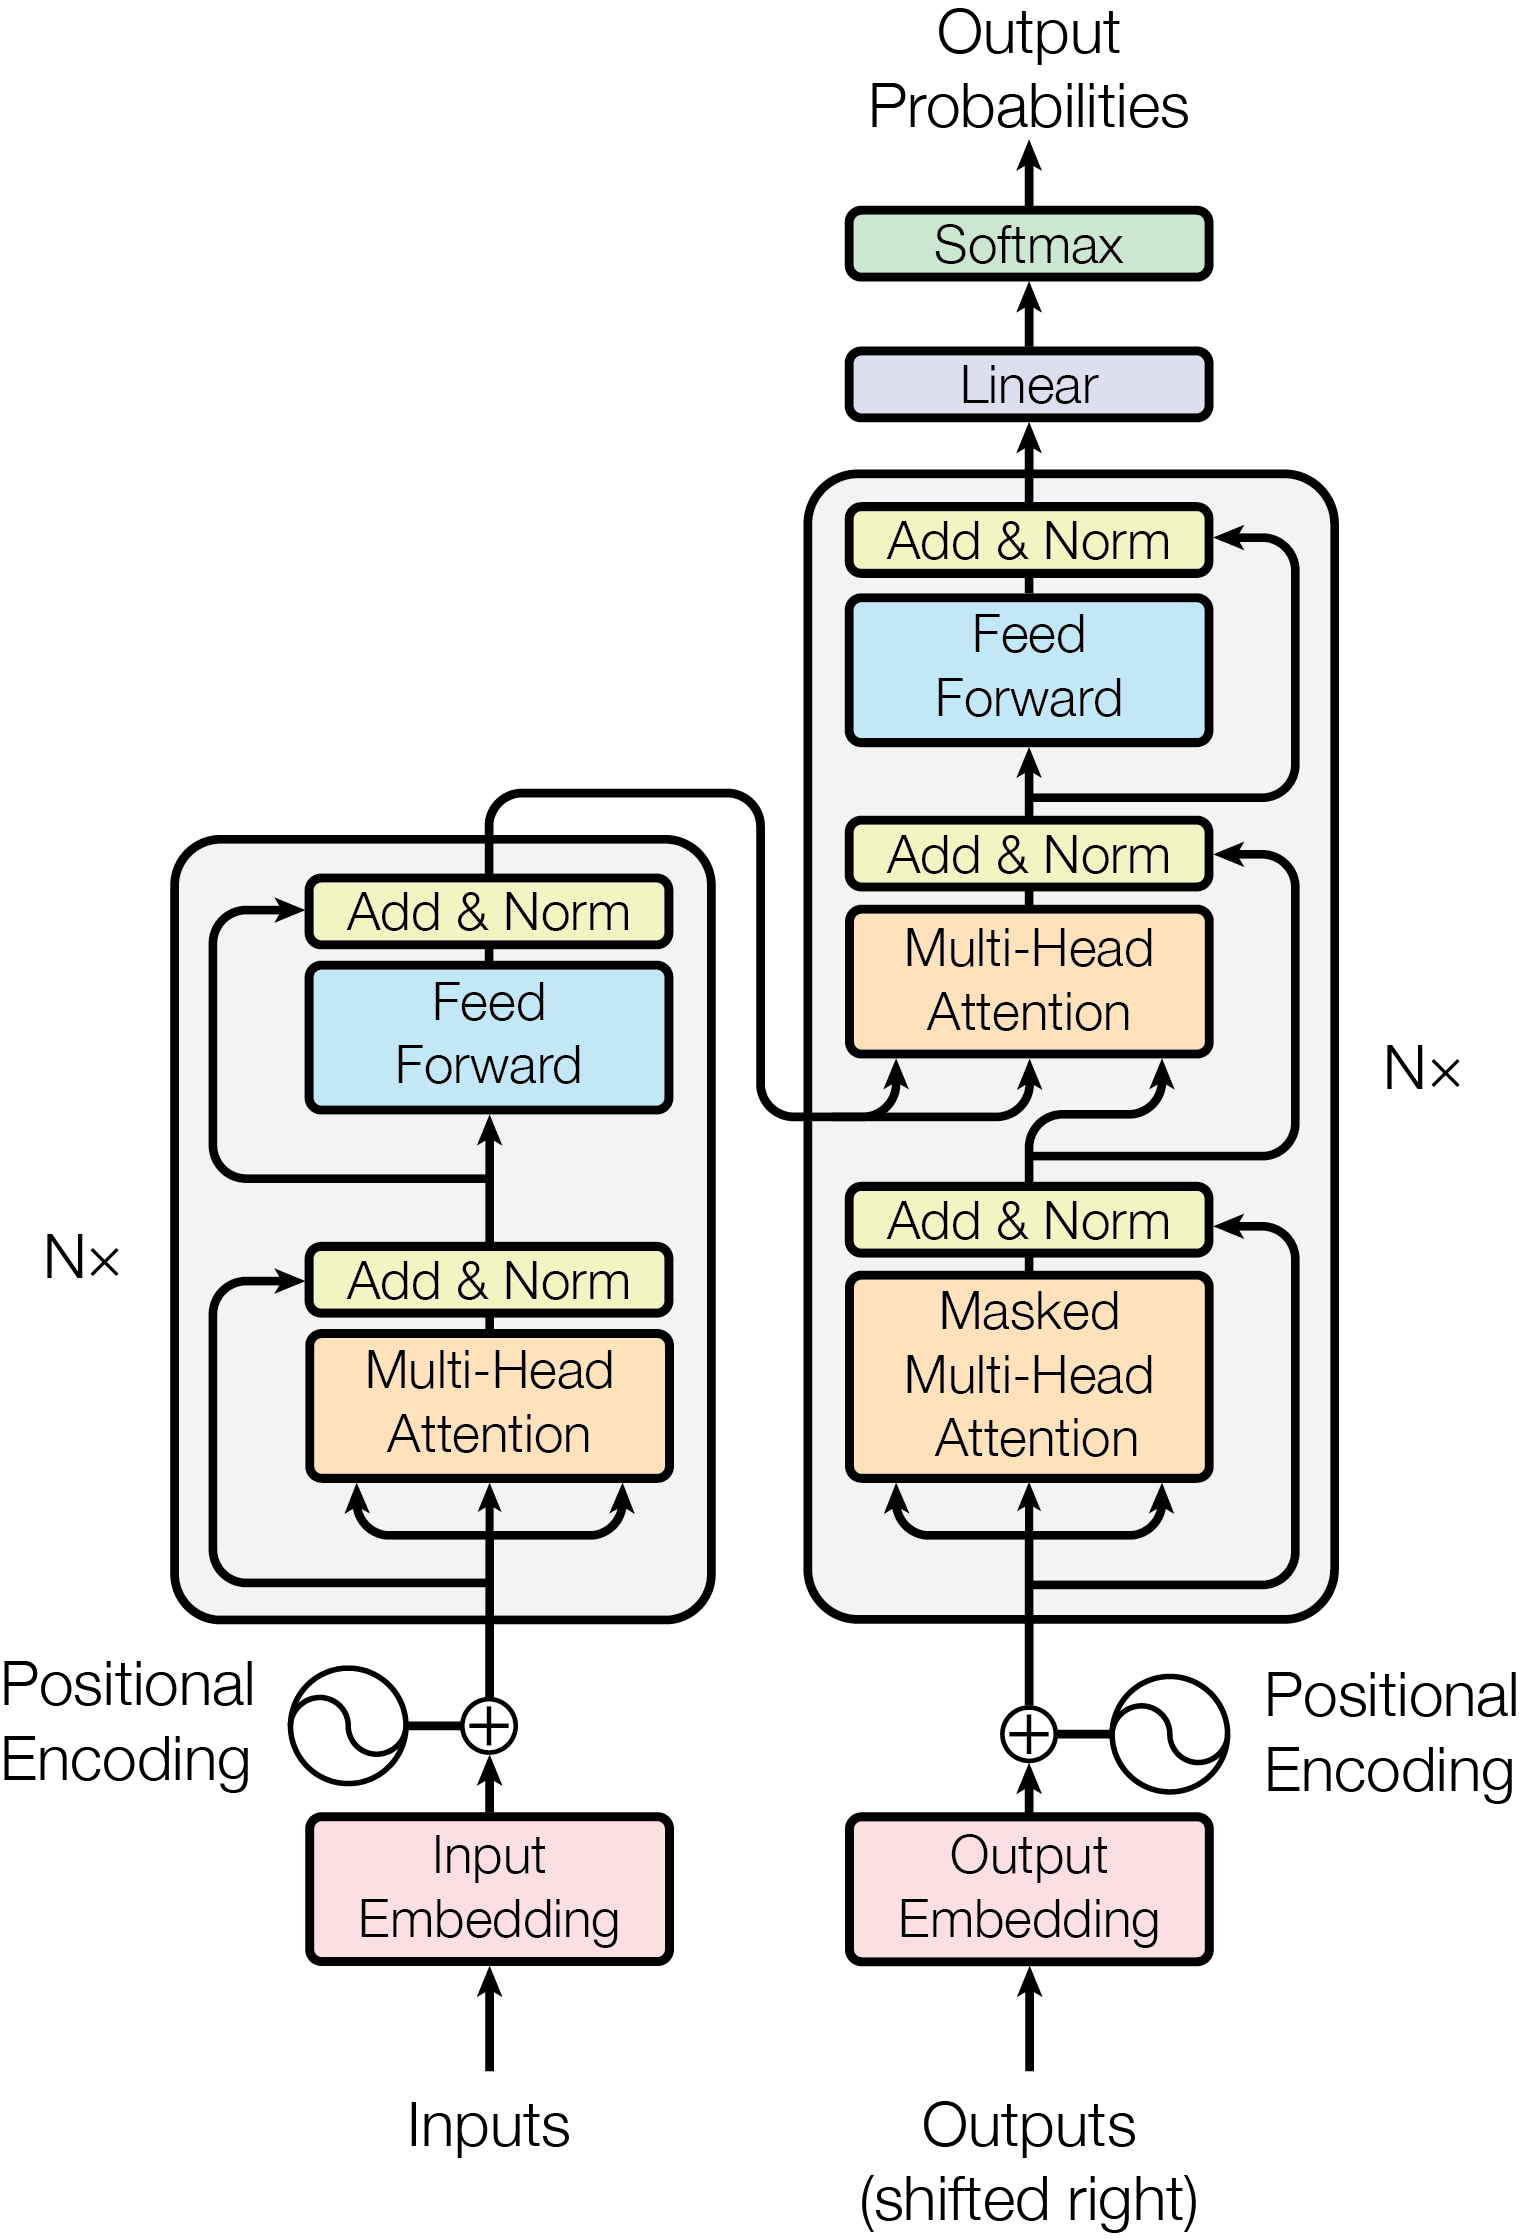
\includegraphics[width=10cm]{gfx/ModalNet-21.png}
    \caption{Architecture Transformer. \cite{vaswani2023attention}}
    \label{fig:transformer-architecture}
\end{figure}

L'architecture Transformer, introduite dans l'article intitulé "Attention is All You Need" par Vaswani et al. en 2017, représente une avancée significative dans le domaine du \ac{nlp} et du \ac{ml}. Cette architecture se distingue par son mécanisme d'attention, permettant aux modèles de pondérer différemment les parties d'une séquence d'entrée lors de la prédiction de la séquence de sortie. Nous aborderons ici les composants clés de l'architecture Transformer ainsi que les formules associées, en nous efforçant de détailler chaque élément avec précision.

\subsubsection{Encodage et Décodage}

\paragraph{Encodeur} \hspace{0pt}

L'encodeur est constitué d'une série de 6 couches identiques. Chaque couche comporte deux sous-couches : la première est un mécanisme d'auto-attention multi-têtes, et la seconde, un réseau de neurones entièrement connecté et positionnel. Un dispositif de connexion résiduelle est utilisé autour de chacune des deux sous-couches, suivi d'une normalisation de couche. Autrement dit, la sortie de chaque sous-couche est le résultat de la normalisation de la somme de l'entrée et du résultat de la sous-couche elle-même. Pour permettre ces connexions résiduelles, toutes les sous-couches du modèle, y compris les couches d'embedding, génèrent des sorties d'une dimension de 512.

\paragraph{Décodeur} \hspace{0pt}

Le décodeur est également formé de 6 couches identiques. En plus des deux sous-couches présentes dans chaque couche de l'encodeur, le décodeur ajoute une troisième sous-couche qui réalise une attention multi-têtes sur la sortie de l'ensemble de l'encodeur. Tout comme dans l'encodeur, des connexions résiduelles sont utilisées autour de chaque sous-couche, suivies d'une normalisation de couche. La sous-couche d'auto-attention du décodeur est également adaptée pour éviter que les positions ne tiennent compte des positions ultérieures. Cette précaution, combinée au décalage des embeddings de sortie d'une position, garantit que les prédictions pour une position donnée ne peuvent dépendre que des sorties connues aux positions précédentes.

\subsubsection{L'attention}
Une fonction d'attention fonctionne en associant une requête à des paires de clés et de valeurs pour produire un résultat, avec tous ces éléments sous forme de vecteurs. Le résultat est obtenu en faisant la somme des valeurs, pondérée par l'importance accordée à chaque valeur. Cette importance est déterminée par une fonction qui mesure à quel point la requête et chaque clé se correspondent.

\begin{figure}
    \begin{minipage}[t]{0.5\textwidth}
      \centering
      Scaled Dot-Product Attention \n
      \vspace{0.5cm}
      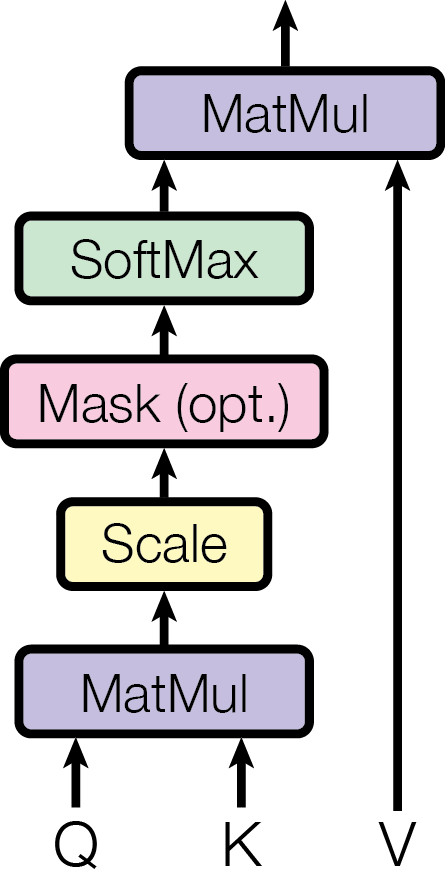
\includegraphics[scale=0.7]{gfx/ModalNet-19}
    \end{minipage}
    \begin{minipage}[t]{0.5\textwidth}
      \centering 
      Multi-Head Attention \n
      \vspace{0.1cm}
      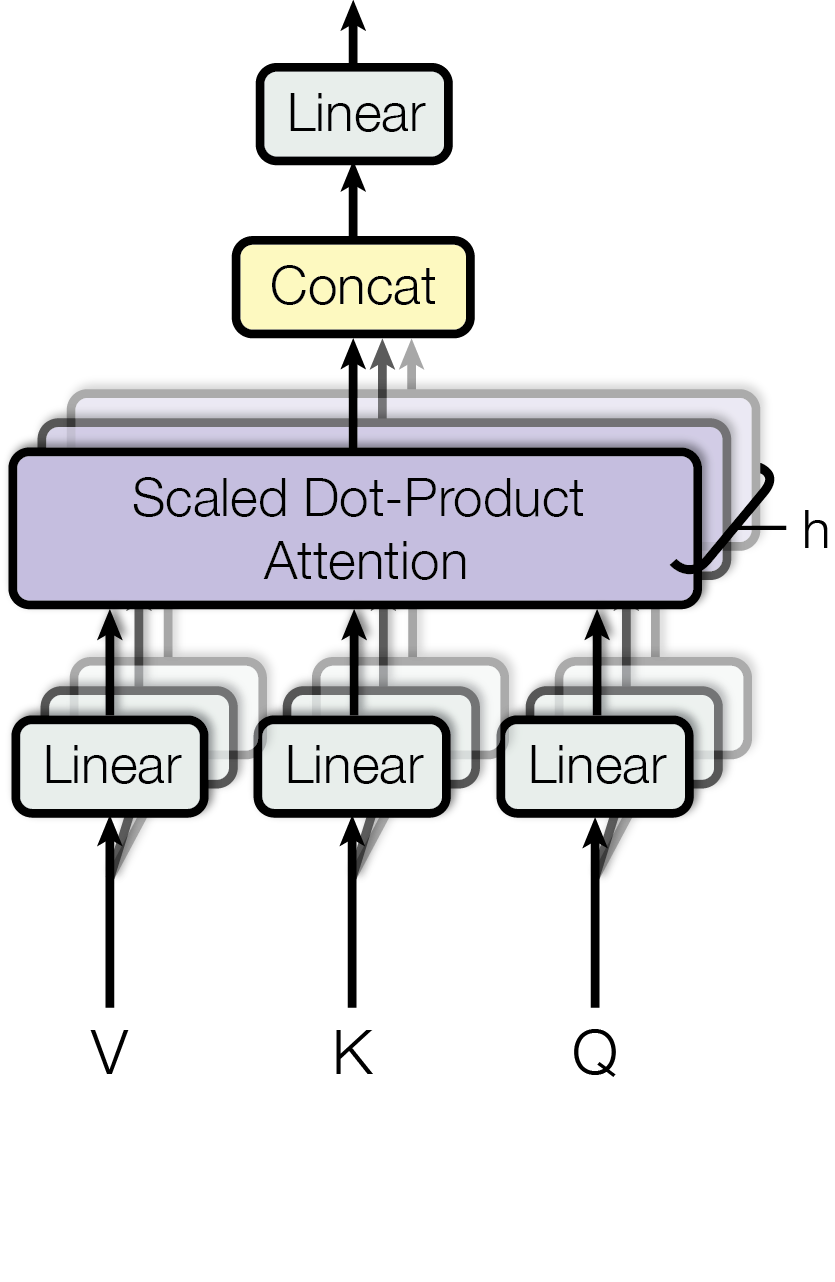
\includegraphics[scale=0.7]{gfx/ModalNet-20}  
    \end{minipage}
    
    \caption{(gauche) Scaled Dot-Product Attention. (droite) Multi-Head Attention consists of several attention layers running in parallel. \cite{vaswani2023attention}}
    \label{fig:multi-head-att}
\end{figure}

\paragraph{Scaled Dot-Product Attention} \hspace{0pt}

Dans l'approche appelée attention par produit scalaire normalisé, l'entrée est composée de requêtes et de clés ayant une dimension \(d_k\), et de valeurs ayant une dimension \(d_v\). Le processus consiste à calculer le produit scalaire de chaque requête avec l'ensemble des clés, puis à diviser chaque résultat par \(\sqrt{d_k}\) avant d'appliquer une fonction softmax pour déterminer les poids attribués aux valeurs.

Habituellement, cette fonction d'attention est calculée pour plusieurs requêtes à la fois, regroupées dans une matrice Q. De même, les clés et les valeurs sont regroupées dans des matrices K et V. La matrice de sortie est alors obtenue par la formule suivante :
\begin{equation}
    \text{Attention}(Q, K, V) = \text{softmax}\left(\frac{QK^T}{\sqrt{d_k}}\right)V
\end{equation}

\paragraph{Multi-Head Attention} \hspace{0pt}

Dans l'approche d'attention multi-têtes, il est courant de ne pas se restreindre à une unique fonction d'attention avec des clés, des valeurs et des requêtes de dimension \(d_{\text{model}}\). Il est avantageux de projeter linéairement les requêtes, les clés et les valeurs plusieurs fois (souvent noté \(h\) fois) avec différentes projections linéaires apprises, vers des dimensions \(d_k\), \(d_k\) et \(d_v\) respectivement. Pour chaque ensemble de projections, la fonction d'attention est appliquée en parallèle, produisant des sorties de dimension \(d_v\). Ces sorties sont ensuite concaténées et projetées à nouveau, aboutissant aux valeurs finales.

L'utilisation de l'attention multi-têtes permet de traiter simultanément des informations provenant de différents sous-espaces de représentation et à différentes positions. Cette méthode surpasse l'approche d'une unique tête d'attention où la moyenne des informations peut limiter la capacité à exploiter ces divers sous-espaces.

La formule générale pour l'attention multi-têtes est définie comme suit :
\begin{equation}
    \text{MultiHead}(Q, K, V) = \text{Concat}(\text{head}_1, ..., \text{head}_h)W^O
\end{equation}

où chaque \(\text{head}_i\) correspond à : 
\begin{equation}
    \text{head}_i = \text{Attention}(QW^Q_i, KW^K_i, VW^V_i)
\end{equation}

Les projections sont réalisées à l'aide de matrices de paramètres spécifiques pour chaque tête, \(W^Q_i \in \mathbb{R}^{d_{\text{model}} \times d_k}\), \(W^K_i \in \mathbb{R}^{d_{\text{model}} \times d_k}\), \(W^V_i \in \mathbb{R}^{d_{\text{model}} \times d_v}\) et \(W^O \in \mathbb{R}^{hd_v \times d_{\text{model}}}\).

\paragraph{Utilisation de l'attention} \hspace{0pt}

L'architecture Transformer utilise l'attention multi-têtes de trois manières distinctes, de premier abord, dans les couches d'attention "encodeur-décodeur", les requêtes proviennent de la couche précédente du décodeur, tandis que les clés et les valeurs de mémoire proviennent de la sortie de l'encodeur. Cela permet à chaque position dans le décodeur de tenir compte de toutes les positions dans la séquence d'entrée, reproduisant ainsi les mécanismes d'attention encodeur-décodeur typiques des modèles de séquence à séquence.

Pour illustrer, prenons l'exemple d'une tâche de traduction d'une phrase juridique de l'Anglais vers le Français. Considérons la phrase "\textit{\textbf{The defendant was acquitted due to lack of evidence}}", à traduire en "\textit{\textbf{L'accusé a été acquitté faute de preuves}}". Lors de la traduction du terme "\textit{preuves}", l'attention encodeur-décodeur va accorder une importance particulière aux mots "\textit{lack}", "\textit{of}" et "\textit{evidence}" de la phrase en anglais, car ils sont essentiels pour rendre le concept d'"\textit{preuve}". En se focalisant sur ces éléments clés, l'attention oriente le modèle vers une traduction plus précise de cette portion du texte juridique

\begin{figure}[H]
    \centering
    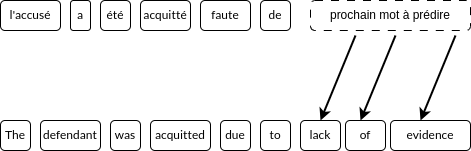
\includegraphics[width=14cm]{gfx/figure-cross-attention-machanism.png}
    \caption[]{L'attention permet de se concentrer sur les parties importantes du texte saisi.}
    \label{fig:cross-attention-mechanism}
\end{figure}

En suite, l'encodeur comprend des couches d'auto-attention. Dans une couche d'auto-attention, les clés, les valeurs et les requêtes proviennent du même endroit, ici, la sortie de la couche précédente de l'encodeur. Chaque position dans l'encodeur peut ainsi tenir compte de toutes les positions dans la couche précédente de l'encodeur.

Pour illustrer, prenons l'exemple de la phrase : \textbf{\textit{"Alice a été félicitée par ses collègues"}}. Imaginons que le modèle cherche à comprendre à qui se réfère le pronom "ses". Grâce à l'auto-attention, le modèle va pondérer différemment les mots de la phrase, en soulignant ceux qui sont significatifs pour "ses" dans ce contexte particulier. Ainsi, dans cet exemple, "Alice" et "collègues" seraient jugés plus importants. L'auto-attention permet au modèle de synthétiser ces mots pour former le concept pertinent, qui pourrait être interprété comme "les collègues d'Alice" dans cette situation.
\begin{figure}[H]
    \centering
    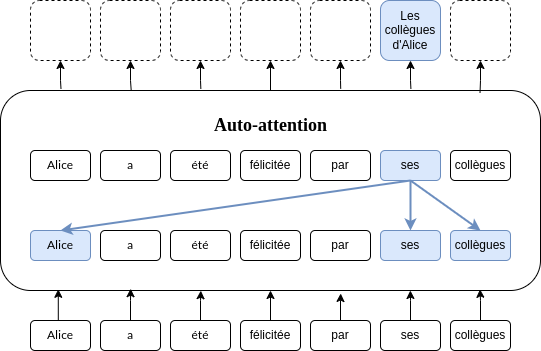
\includegraphics[width=12cm]{gfx/figure-self-attention.png}
    \caption[]{L'auto-attention permet l'émergence du concept de "collègues d'Alice". \cite{Caelen_Blete_2023}}
    \label{fig:attention-vs-multihead}
\end{figure}

Enfin, De manière similaire, les couches d'auto-attention dans le décodeur permettent à chaque position du décodeur de prendre en compte toutes les positions dans le décodeur jusqu'à la position actuelle incluse. Il est nécessaire de bloquer le flux d'informations vers la gauche dans le décodeur pour préserver la propriété auto-régressive. Cela est réalisé au sein de l'attention par produit scalaire normalisé en masquant (en réglant à $-\infty$) toutes les valeurs dans l'entrée du softmax qui correspondent à des connexions interdites.

\subsubsection{Position-wise Feed-Forward Networks}

En plus des sous-couches d'attention, chaque couche de l'encodeur et du décodeur intègre un réseau de neurones entièrement connecté, appliqué séparément et de manière identique à chaque position. Ce réseau est composé de deux transformations linéaires avec une activation ReLU entre les deux. La fonction du réseau de neurones peut être décrite par la formule suivante : 
\begin{equation}
    \text{FFN}(x) = \max(0, xW_1 + b_1)W_2 + b_2
\end{equation}

où \( \max(0, z) \) représente la fonction d'activation ReLU appliquée élément par élément au vecteur \( z \).

Même si les transformations linéaires sont identiques pour les différentes positions, elles utilisent des paramètres distincts d'une couche à l'autre. Cela peut également être vu comme l'équivalent de deux convolutions de taille de noyau 1. La dimension des entrées et des sorties est \( d_{\text{model}} = 512 \), tandis que la dimension de la couche intermédiaire est \( d_{\text{ff}} = 2048 \).

\subsubsection{Embeddings et Softmax}
Comme dans d'autres modèles de transduction de séquence, des embeddings appris sont utilisés pour convertir les tokens d'entrée et de sortie en vecteurs de dimension \(d_{\text{model}}\). Une transformation linéaire apprise suivie d'une fonction softmax est également employée pour convertir la sortie du décodeur en probabilités du prochain token prédit. Dans ce modèle, la même matrice de poids est partagée entre les deux couches d'embedding et la transformation linéaire précédant la softmax, à l'instar d'autres travaux référencés. Dans les couches d'embedding, ces poids sont multipliés par \(\sqrt{d_{\text{model}}}\) pour ajuster l'échelle.

\subsubsection{Positional Encoding}
Dans les modèles de traitement de séquences qui ne reposent ni sur des mécanismes de récurrence ni sur des convolutions, il est crucial d'intégrer une forme de connaissance sur l'ordre des éléments de la séquence. Pour cela, des "encodages positionnels" sont ajoutés aux vecteurs d'embeddings en début de l'encodeur et du décodeur. Ces encodages ont la même dimension que les embeddings, ce qui permet de les additionner ensemble. Il existe plusieurs méthodes pour créer ces encodages, qu'ils soient définis à l'avance ou appris durant l'entraînement.

Une méthode courante consiste à utiliser des fonctions sinus et cosinus avec des fréquences variées pour générer ces encodages positionnels. La formule pour un encodage positionnel est la suivante : pour une position \(pos\) dans la séquence et pour chaque dimension \(i\) de l'encodage, la valeur est donnée par une fonction sinus pour les dimensions paires et cosinus pour les dimensions impaires, avec une fréquence qui décroît exponentiellement le long des dimensions.

Cette approche a été choisie car elle facilite l'apprentissage de la relation entre des positions relatives dans la séquence. En effet, un décalage fixe entre deux positions peut être représenté par une transformation linéaire des encodages, ce qui simplifie le traitement par le modèle.

Bien que des tests aient été effectués avec des encodages positionnels appris, les résultats obtenus étaient très similaires à ceux obtenus avec les encodages sinusoidaux. La préférence pour les encodages sinusoidaux est motivée par leur potentiel à mieux généraliser pour des séquences plus longues que celles rencontrées lors de l'entraînement, offrant ainsi une plus grande flexibilité au modèle.

% %---------------------------------------------------------------------------------------%
\subsection{Résumé de l'évolution des chatbots}
\label{ch:1:section:history}

L'aventure du \acf{nlp} et de l'\acf{ia} dans le domaine des chatbots est une histoire captivante de progrès technologique et d'innovation humaine. Le terme "chatbot" lui-même, une contraction de "chat" et "robot", trouve ses origines dans sa fonction initiale de système de dialogue textuel simulant le langage humain. Ces premières versions, essentiellement des programmes informatiques, utilisaient des interfaces d'entrée et de sortie pour simuler une expérience utilisateur mobile évoquant une conversation en temps réel. Toutefois, l'évolution des chatbots a largement dépassé cette interaction textuelle de base \cite{alamin2024history}.

L'histoire du développement des chatbots et de l'intelligence artificielle (IA) dans la communication entre humains et machines est une saga captivante, jalonnée d'innovations technologiques et d'avancées majeures qui ont révolutionné notre interaction avec les machines. Dès 1906, les chaînes de Markov \cite{Green1996MarkovCM}, inventées par le mathématicien russe Andrey Markov, ont jeté les bases de la prédiction de séquences aléatoires, permettant d'enseigner aux machines la création de données nouvelles, une première étape essentielle vers l'exploration du potentiel des chatbots.

L'aventure s'accélère en 1950 avec la proposition du test de Turing par Alan Turing \cite{turingTest}, évaluant l'intelligence d'une machine à travers sa capacité à imiter le langage humain, un tournant décisif inspirant des décennies de recherche. L'apparition d'ELIZA \cite{eliza1966} en 1966, conçue par Joseph Weizenbaum, marque la naissance des premiers chatbots, malgré une compréhension et une interaction encore limitées. L'évolution continue avec PARRY en 1972, simulant un patient schizophrène paranoïaque, offrant une nouvelle perspective sur les interactions conversationnelles. Les décennies suivantes voient la création de Racter et Jabberwacky, explorant respectivement la génération aléatoire de texte et l'apprentissage à partir d'interactions en ligne, des pas de géant vers des chatbots plus interactifs et personnalisés \cite{chatbotHistoryChatbots, Weizenbaum1966ELIZAaCP, alamin2024history}. 

Le champ du \ac{ml} a connu une avancée significative au début des années 2000 avec l'introduction de l'apprentissage profond et l'arrivée d'Internet, permettant aux ordinateurs de comprendre et d'interpréter l'information sous diverses formes. Cette période a vu les grandes entreprises technologiques pousser le progrès de l'intelligence artificielle, en utilisant la puissance computationnelle pour relever des défis complexes, avec des projets comme CALO qui pavent la voie à des assistants virtuels sophistiqués tels que Siri \cite{siri}, marquant l'aube d'une nouvelle ère dans L'\ac{ia} conversationnelle.

L'introduction de \acfp{llm} par OpenAI avec GPT et ses versions successives, ainsi que l'annonce de Google Bard (aujourd'hui Gemini), témoignent d'une évolution rapide vers des chatbots dotés d'une compréhension contextuelle et d'une capacité de raisonnement avancées, reflétant l'incroyable voyage depuis les premières techniques de correspondance de motifs à l'utilisation des architectures neurales Transformer (voir Section~\ref{ch:1:section:transformer}).

% %---------------------------------------------------------------------------------------%
\newpage
\section{Généralités sur le Droit Congolais}
\label{ch:1:section:introduction-law}

Le droit, tel qu'il est envisagé par le Professeur Ilunga, est compris comme une règle de conduite sociale dont le respect est garanti par l'autorité publique. Cette définition met en lumière le rôle fondamental du Droit dans l'organisation de la société, en établissant des normes de comportement obligatoires pour ses membres. Le Droit existe dès l'instant où il y a société, soulignant l'adage « Ubi societas, ibi ius » (Là où il y a une société, il y a du Droit).

Cette perspective révèle le Droit non seulement comme un ensemble de règles coercitives mais aussi comme un phénomène vivant, qui naît, évolue et meurt au gré des changements sociétaux. Par conséquent, le Droit régit non seulement les rapports économiques et les interactions entre individus et État, mais s'étend aussi à des domaines aussi personnels que les relations familiales, illustrant sa présence omniprésente et son influence sur tous les aspects de la vie humaine .

le Droit en \ac{rdc}, ainsi que dans toute société, s'avère être une structure complexe et dynamique, adaptative aux évolutions des rapports humains et aux exigences de justice et d'ordre social.

\subsection{Le système juridique Congolais}
Pour aborder le thème du système juridique congolais, nous examinerons d'abord ce qu'est un système juridique, comment il est constitué, et comment cela s'applique spécifiquement à la \acf{rdc}. 

Un système juridique est l'ensemble organisé des règles de droit applicables dans un espace géographique donné, régissant les rapports entre les personnes ainsi que ceux entre les personnes et l'État. Il comprend la structure institutionnelle chargée de créer, interpréter, et appliquer ces règles. Les systèmes juridiques se classifient généralement en différentes familles de droit, en fonction de leurs origines historiques, de leurs caractéristiques communes et de leurs principes fondateurs.

Il est évident que la distinction entre \textbf{le Droit objectif} et \textbf{le droit subjectif} est fondamentale. Le Droit objectif désigne l'ensemble des règles de Droit qui régissent les rapports sociaux et s'appliquent de manière impersonnelle, tandis que les droits subjectifs représentent les prérogatives spécifiques accordées aux individus ou entités, leur permettant de faire valoir leurs droits dans des situations concrètes.

Au niveau des sources formelles du Droit en \ac{rdc}, la loi et la coutume apparaissent comme des piliers fondamentaux. La loi, dans son sens le plus large, englobe divers actes normatifs allant de la constitution aux ordonnances et décrets, caractérisés par leur impersonnalité, leur obligatorité, et leur permanence. La coutume, quant à elle, bien qu'elle doive céder devant la loi écrite, joue encore un rôle important, notamment dans des domaines moins réglementés par le Droit écrit.

La notion de droits subjectifs en Droit congolais est explorée à travers leur classification et leur preuve. Ces droits, attachés à l'individu, peuvent être patrimoniaux ou extrapatrimoniaux, reflétant respectivement des intérêts évaluables en argent et ceux qui ne le sont pas. Les droits patrimoniaux englobent, entre autres, les droits réels (comme la propriété) et les droits de créance, tandis que les droits extrapatrimoniaux incluent des droits tels que le droit à la vie, à la liberté, et au respect de la vie privée.

Le système juridique de la RDC s'inscrit dans la famille du droit civil, héritage du colonialisme belge. Cette influence se manifeste dans la prédominance du droit écrit et dans l'organisation judiciaire du pays. Néanmoins, la coutume occupe toujours une place significative, surtout en matière de droit de la famille et de droit foncier, où elle coexiste avec les règlements nationaux et internationaux. Cette coexistence illustre la complexité du système juridique Congolais, où les sources formelles et matérielles du droit, ainsi que les droits subjectifs et leur application, reflètent un mélange d'influences traditionnelles et modernes.

L'application de ce système juridique en RDC montre un équilibre entre le respect des normes internationales et la reconnaissance des spécificités locales. Cela est particulièrement visible dans le domaine des droits de l'homme, où les engagements internationaux de la RDC se conjuguent avec les réalités et pratiques locales pour façonner l'application des droits subjectifs dans le pays.


\subsection{Aperçu du Cadre Législatif Congolais}

Pour approfondir l'aperçu du cadre législatif congolais, nous allons définir ce qu'est une loi, présenter les différentes sortes de lois existantes dans le système juridique de la \ac{rdc} et expliquer comment une loi y est élaborée.

Une loi est définie comme une règle de conduite sociale, obligatoire, qui émane de l'autorité publique. Elle est d'application générale et permanente, pouvant être impérative ou supplétive. La loi au sens strict émane du Parlement, tandis que la loi au sens large inclut également les règlements, les contrats, et d'autres formes de textes normatifs .

Le système juridique congolais comprend plusieurs sortes de lois, chacune ayant sa spécificité et sa hiérarchie au sein de l'ordre juridique. Voici un tableau récapitulatif des sortes de lois, adaptées à la \ac{rdc}:

\begin{table}[h]
\centering
\begin{tabular}{|l|p{10.5cm}|}
\hline
\textbf{Type de Loi} & \textbf{Description} \\ \hline
Loi Constitutionnelle & La charte ou loi fondamentale de l'État, suprême sur le reste du droit \\ \hline
Lois Organiques & Relatives à l'organisation et fonctionnement des pouvoirs publics \\ \hline
Lois Ordinaires & Établies par le Parlement dans son domaine de compétence \\ \hline
Lois-Cadre & Définissent les grands principes d'une réforme, détaillée ensuite par le pouvoir réglementaire \\ \hline
Règlements & Actes de portée générale et impersonnelle édictés par l'exécutif \\ \hline
\end{tabular}
\caption{Sortes de Lois dans le Système Juridique de la RDC}
\end{table}

Cet ajustement présente le même contenu mais dans un format légèrement différent, qui peut être plus familier ou approprié pour certains usages documentaires ou de présentation. Les différentes catégories de lois sont conçues pour structurer l'organisation de l'État, réguler la vie en société, et fournir un cadre pour l'administration publique.


\paragraph{Élaboration d'une Loi} \hspace{0pt}

L'élaboration d'une loi en RDC suit un processus bien défini, impliquant différentes étapes et acteurs du système juridique et politique. Ce processus commence généralement par l'initiative législative, qui peut être prise par les membres du Parlement, le gouvernement, ou par voie de pétition populaire dans certains cas \footnote{\href{https://www.memoireonline.com/12/12/6552/Problematique-du-droit-de-la-petition-dans-la-constitution-du-18-fevrier-2006-de-la-RDC.html}{Problématique du droit de la pétition dans la constitution du 18 février 2006 de la RDC}}. Une fois proposée, une loi doit passer par diverses étapes de discussion, d'amendement, et d'approbation dans les deux chambres du Parlement congolais.

Après l'approbation par le Parlement, la loi est soumise au Président de la République pour promulgation et publication au Journal Officiel, devenant ainsi exécutoire. Ce processus d'élaboration législative est conçu pour assurer la participation démocratique, le débat ouvert, et la réflexion approfondie sur les propositions législatives avant qu'elles ne deviennent des lois.

\paragraph{La pyramide de Kelsen \cite{Kelsen_Raphael_2024, Kelsen_jurixio_2023}} \hspace{0pt}

\begin{figure}[H]
    \centering
    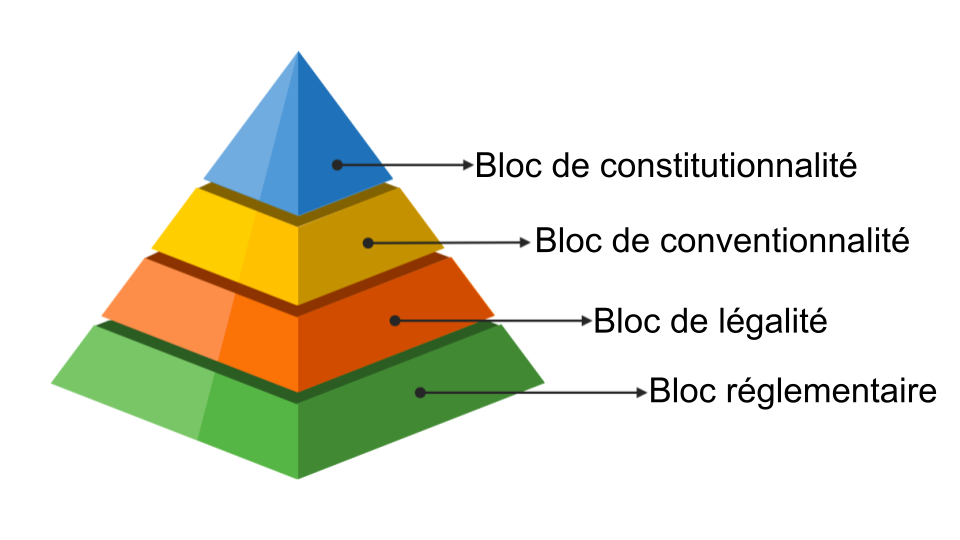
\includegraphics[width=12cm]{gfx/fig-law-pyramide.png}
    \caption{La pyramide de Kelsen permet de visualiser la hiérarchie des normes. \cite{frwiki:212163472}}
    \label{fig:datagenerated}
\end{figure}

La pyramide de Kelsen est un concept essentiel pour comprendre la structure et la hiérarchie des normes juridiques dans un système juridique, y compris celui de la République Démocratique du Congo. Développée par le juriste Hans Kelsen \footnote{"Hans Kelsen, né le 11 octobre 1881 à Prague et mort le 19 avril 1973 à Orinda, est un juriste austro-américain, fils d'une famille juive de Bohême et de Galicie. Théoricien du droit, il est l'auteur de la « Théorie pure du droit », œuvre phare de la discipline." \cite{frwiki:213425509}}, cette théorie illustre comment les différentes règles de droit s'ordonnent et se subordonnent les unes aux autres, formant une structure pyramidale.

Au sommet de cette pyramide se trouve la Constitution, qui est la norme suprême d'un pays. Toutes les autres normes juridiques dérivent de la Constitution et doivent lui être conformes. En RDC, comme dans de nombreux autres systèmes juridiques, la Constitution détermine les principes fondamentaux de l'État, les droits et libertés des citoyens, ainsi que l'organisation et le fonctionnement des pouvoirs publics.

Sous la Constitution, on trouve les lois organiques qui ont une valeur supérieure aux lois ordinaires. Les lois organiques précisent l'organisation et le fonctionnement des institutions prévues par la Constitution. Elles sont suivies des lois ordinaires qui régissent les aspects spécifiques de la vie sociale, économique, et juridique.

Les règlements exécutifs, comprenant les décrets et les arrêtés, viennent ensuite. Ces actes sont émis par le pouvoir exécutif pour assurer l'application des lois. Bien qu'inférieurs aux lois, ils jouent un rôle crucial dans la mise en œuvre des politiques publiques et des législations.

Enfin, à la base de la pyramide, se trouvent les normes réglementaires locales et les décisions de jurisprudence. Ces dernières, bien que ne constituant pas une source de droit formelle dans tous les systèmes juridiques, influencent significativement l'application et l'interprétation du droit.

La pyramide de Kelsen met en lumière la notion d'ordre juridique, où chaque norme tire sa validité de la norme immédiatement supérieure, jusqu'à la Constitution qui est la source ultime de toute validité juridique. Ce principe de hiérarchie des normes assure la cohérence et la systématicité du droit, permettant ainsi de prévenir les conflits normatifs et de garantir une certaine prévisibilité et stabilité dans l'ordre juridique.

\newpage
\section{Intersection entre Intelligence artificielle et Droit}

L'intersection entre l'\acf{ia} et le droit représente un domaine d'étude fascinant et en constante évolution, reflétant l'intégration croissante des technologies avancées dans tous les aspects de la société. Alors que l'\ac{ia} continue de progresser à un rythme exponentiel, son impact sur le domaine juridique devient de plus en plus significatif, soulevant à la fois des opportunités et des défis uniques pour les praticiens, les législateurs et les institutions juridiques.

L'application de l'\ac{ia} dans le droit ouvre la voie à une multitude d'innovations, allant de l'automatisation des tâches documentaires à la prédiction des issues judiciaires, en passant par l'amélioration de l'accès à la justice. Ces technologies promettent d'accroître l'efficacité des processus légaux, de réduire les coûts et d'améliorer la qualité des services juridiques. Par exemple, les chatbots juridiques peuvent fournir des consultations préliminaires, tandis que les systèmes de traitement du langage naturel permettent d'analyser rapidement d'importants volumes de textes juridiques pour extraire des informations pertinentes.

Toutefois, l'adoption de l'\ac{ia} dans le secteur juridique n'est pas sans soulever des questions complexes relatives à l'éthique, à la responsabilité, à la transparence et à la protection des données personnelles. Les systèmes d'\ac{ia}, bien qu'incroyablement puissants, peuvent présenter des biais, des erreurs et des limitations qui, s'ils ne sont pas correctement adressés, pourraient compromettre les droits et libertés fondamentales des individus. En outre, l'émergence de l'\ac{ia} générative et des modèles \ac{llm} pose de nouvelles interrogations sur les droits de propriété intellectuelle, notamment la paternité et la titularité des œuvres créées par ou avec l'aide de l'\ac{ia}.

Face à ces enjeux, le monde juridique est appelé à réfléchir et à adapter ses cadres législatifs pour encadrer l'utilisation de l'\ac{ia}, garantissant ainsi que son déploiement se fasse dans le respect des principes de justice, d'équité et de respect de la vie privée. Cette tâche implique une collaboration étroite entre juristes, technologues, chercheurs et décideurs politiques pour élaborer des normes et des régulations qui équilibrent les avantages de l'\ac{ia} avec la protection des droits fondamentaux.

L'\ac{ia} et du droit a conduit à une variété d'applications tant dans la recherche que dans l'industrie, notamment à travers le développement et le déploiement de services web innovants. Ces applications illustrent comment l'\ac{ia} peut transformer les pratiques juridiques, offrir de nouveaux outils pour l'analyse et la gestion des données légales, et même réinventer l'accès à la justice pour le grand public.

\newpage
\subsection{Dans la recherche}

\begin{table}[h]
\centering
\begin{tabular}{|m{0.3\textwidth}|m{0.65\textwidth}|}
\hline
\textbf{Article} & \textbf{Résumé} \\
\hline
Development of a Legal Document AI-Chatbot & Cet article présente le développement d'un chatbot AI pour la documentation juridique, exploitant le potentiel de L'\ac{ia}, notamment des chatbots, pour simplifier la gestion des documents légaux. Le chatbot fonctionne en traitant les requêtes dans le contexte des documents chargés sur le serveur et en fournissant des réponses pertinentes \cite{devaraj2023development}. \\
\hline
ChatLaw: Open-Source Legal Large Language Model with Integrated External Knowledge Bases & ChatLaw est un modèle de langage large open-source conçu pour le domaine juridique chinois, visant à résoudre le problème des hallucinations du modèle lors de la récupération de données de référence. Le modèle intègre une base de connaissances externe pour améliorer la précision des réponses et est ouvert à la contribution communautaire \cite{cui2023chatlaw}. \\
\hline
Generative AI and US Intellectual Property Law & Cet article aborde les implications juridiques et éthiques de L'\ac{ia} générative sur les droits d'auteur, la production de contenu, la collecte de données, la précision de l'information et les droits de propriété intellectuelle, en se concentrant sur les défis posés par les systèmes d'\ac{ia} générative aux droits des créateurs de contenu humains dans le contexte du droit de la propriété intellectuelle aux États-Unis \cite{poland2023generative}. \\
\hline
\end{tabular}
\caption{Résumé des articles sur l'\acf{ia} pour des applications juridiques}
\label{tab:law-article}
\end{table}

Chaque jour, de nouvelles publications émergent, poussant les frontières de ce que ces technologies peuvent accomplir dans le secteur juridique.

\newpage
\subsection{Dans l'industrie}

\begin{table}[h]
    \centering
    \begin{tabular}{|l|p{12cm}|}
        \hline
        \textbf{Service} & \textbf{Description} \\
        \hline
        \href{https://legalmasterai.com/}{LegalMasterAI} & Plateforme d'automatisation des tâches juridiques basée sur L'\ac{ia} \\
        \hline
        \href{https://ailawyer.pro/fr}{AI Lawyer} & Assistant juridique personnel basé sur L'\ac{ia} pour les recherches et formalités administratives \\
        \hline
        \href{https://www.legalai.io/}{LegalAI} & Plateforme mondiale d'intelligence juridique avec accès à une vaste collection d'informations juridiques \\
        \hline
        \href{https://vlex.com/}{vLex} & Collection d'informations juridiques provenant de 100 pays \\
        \hline
        \href{https://www.harvey.ai/}{Harvey} & Modèles linguistiques juridiques personnalisés pour les cabinets d'avocats \\
        \hline
        \href{https://lawchatgpt.com/}{LawChatGPT} & Outil d'\ac{ia} pour des réponses juridiques en langage naturel \\
        \hline
        \href{https://www.ai.law/}{AI.law} & Solutions d'automatisation juridique basées sur L'\ac{ia} \\
        \hline
        \href{https://juro.com/ai}{Juro} & Plateforme d'automatisation des contrats \\
        \hline
        \href{https://www.lexisnexis.com/en-us/products/lexis-plus-ai.page}{LexisNexis} & Solutions d'\ac{ia} pour la recherche juridique et l'analyse des litiges \\
        \hline
        \href{https://www.paxton.ai/}{Paxton} & Plateforme d'automatisation des contrats pour accélérer le processus de rédaction et d'examen \\
        \hline
        \href{https://www.luminance.com/}{Luminance} & Analyse de documents juridiques basée sur L'\ac{ia} \\
        \hline
        \href{https://www.robinai.com/}{RobinAI} & Automatisation des contrats \\
        \hline
        \href{https://www.spellbook.legal/}{Spellbook Legal} & Automatisation des contrats avec recherche de clauses contractuelles \\
        \hline
        \href{https://www.superlegal.ai/}{SuperLegalAI} & Automatisation des tâches juridiques avec recherche de jurisprudence et rédaction de contrats \\
        \hline
    \end{tabular}

    \caption{Résumé des services et applications web d'\acf{ia} pour des applications juridiques}
    \label{table:law-ai-tool}
\end{table}



% %--------------------------------------------------------------------------------------------------------%
\section{Conclusion}

Ce chapitre a fourni une vue d'ensemble approfondie des modèles \ac{llm}, en mettant en lumière les avancées récentes, les applications marquantes et les défis associés, avec un accent particulier sur les applications juridiques et les chatbots. Grâce à cette exploration, nous avons établi un cadre théorique et contextuel essentiel pour comprendre l'innovation et la pertinence de ce mémoire dans le domaine de l'intelligence artificielle appliquée au droit. 

En conclusion, les perspectives offertes par les \ac{llm} dans le domaine juridique sont vastes et prometteuses, marquant le début d'une nouvelle ère dans laquelle l'intelligence artificielle jouera un rôle central dans la transformation et l'amélioration des services juridiques. Ce mémoire, en explorant ces technologies et leurs applications, aspire à contribuer à cette évolution, en mettant en évidence les opportunités et en naviguant à travers les défis inhérents à cette intégration pionnière.